\documentclass[aspectratio=169]{beamer}

\usepackage{ctex}
\usepackage{hyperref}
\usepackage{graphicx}
\usepackage{booktabs}
\usepackage{tabularx}
\usepackage{array}
\usepackage{xcolor}
\usepackage[blue]{WHUBeamer}

\title[WikiBridge]{\textbf{WikiBridge}}
\subtitle{零代码本地知识库编译与公网发布平台}
\institute{武汉大学}
\date{\today}

\newcommand{\keypoint}[1]{\textcolor{whu}{\textbf{#1}}}
\AtBeginSection[]{}

\begin{document}

\begin{frame}
    \titlepage
    \begin{figure}
        \centering
        
\includegraphics[width=0.22\linewidth]{pic/dark.pdf}
    \end{figure}
\end{frame}

\begin{frame}{汇报提纲}
    \tableofcontents[sectionstyle=show,subsectionstyle=show/shaded/hide]
\end{frame}

\section{选题背景}

\begin{frame}{为什么需要 WikiBridge？}
    \begin{block}{三类核心痛点}
        \begin{itemize}
            \item \keypoint{知识零散难归档}：文档、网页、笔记和聊天记录分散，难以沉淀为可复用知识。
            \item \keypoint{AI 知识库门槛高}：现有 RAG 方案依赖环境配置、模型服务和数据库。
            \item \keypoint{本地共享困难}：本地知识库很难低成本、安全地发布到公网供他人访问。
        \end{itemize}
    \end{block}

    \vspace{0.25cm}
    \begin{alertblock}{阶段选题}
        面向低技术门槛用户，构建一个从本地资料整理到公网访问的零代码知识库发布工具。
    \end{alertblock}
\end{frame}

\begin{frame}{选题价值：本地编译，轻量分发}
    \small
    \begin{tabularx}{\textwidth}{>{\raggedright\arraybackslash}p{0.2\textwidth}X}
        \toprule
        \textbf{环节} & \textbf{价值} \\
        \midrule
        素材输入 & 用户将 Word、PDF、网页摘录放入本地素材箱。 \\
        LLM-Wiki 编译 & 大模型 Agent 提炼、去重，生成双向链接 Markdown Wiki。 \\
        frp 无感发布 & 本地静态站点通过后台隧道映射为公网 URL。 \\
        浏览器消费 & 外部用户直接浏览知识图谱，并通过 Chatbox 问答。 \\
        \bottomrule
    \end{tabularx}

    \vspace{0.35cm}
    \centering
    \keypoint{本地保存数据与计算} $\rightarrow$
    \keypoint{云端只做账号、鉴权和流量调度}
\end{frame}

\section{需求分析}

\begin{frame}{核心功能需求：三端拆分}
    \small
    \begin{tabularx}{\textwidth}{>{\raggedright\arraybackslash}p{0.18\textwidth}p{0.42\textwidth}X}
        \toprule
        \textbf{端} & \textbf{核心能力} & \textbf{阶段目标} \\
        \midrule
        用户端 GUI & 登录、素材箱、Add / Compile / Lint、静态站托管、公网 URL。 & 零代码生成与发布知识库。 \\
        服务器管理面板 & 用户认证、Token 鉴权、端口 / 子域名分配、frps 状态。 & 只管控制面，不保存知识内容。 \\
        知识库消费端 & 静态 Wiki 浏览、双向链接、Chatbox、引用展示。 & 外部访问者用浏览器直接使用。 \\
        \bottomrule
    \end{tabularx}
\end{frame}

\begin{frame}{用例图：角色与系统边界}
    \begin{figure}
        \centering
        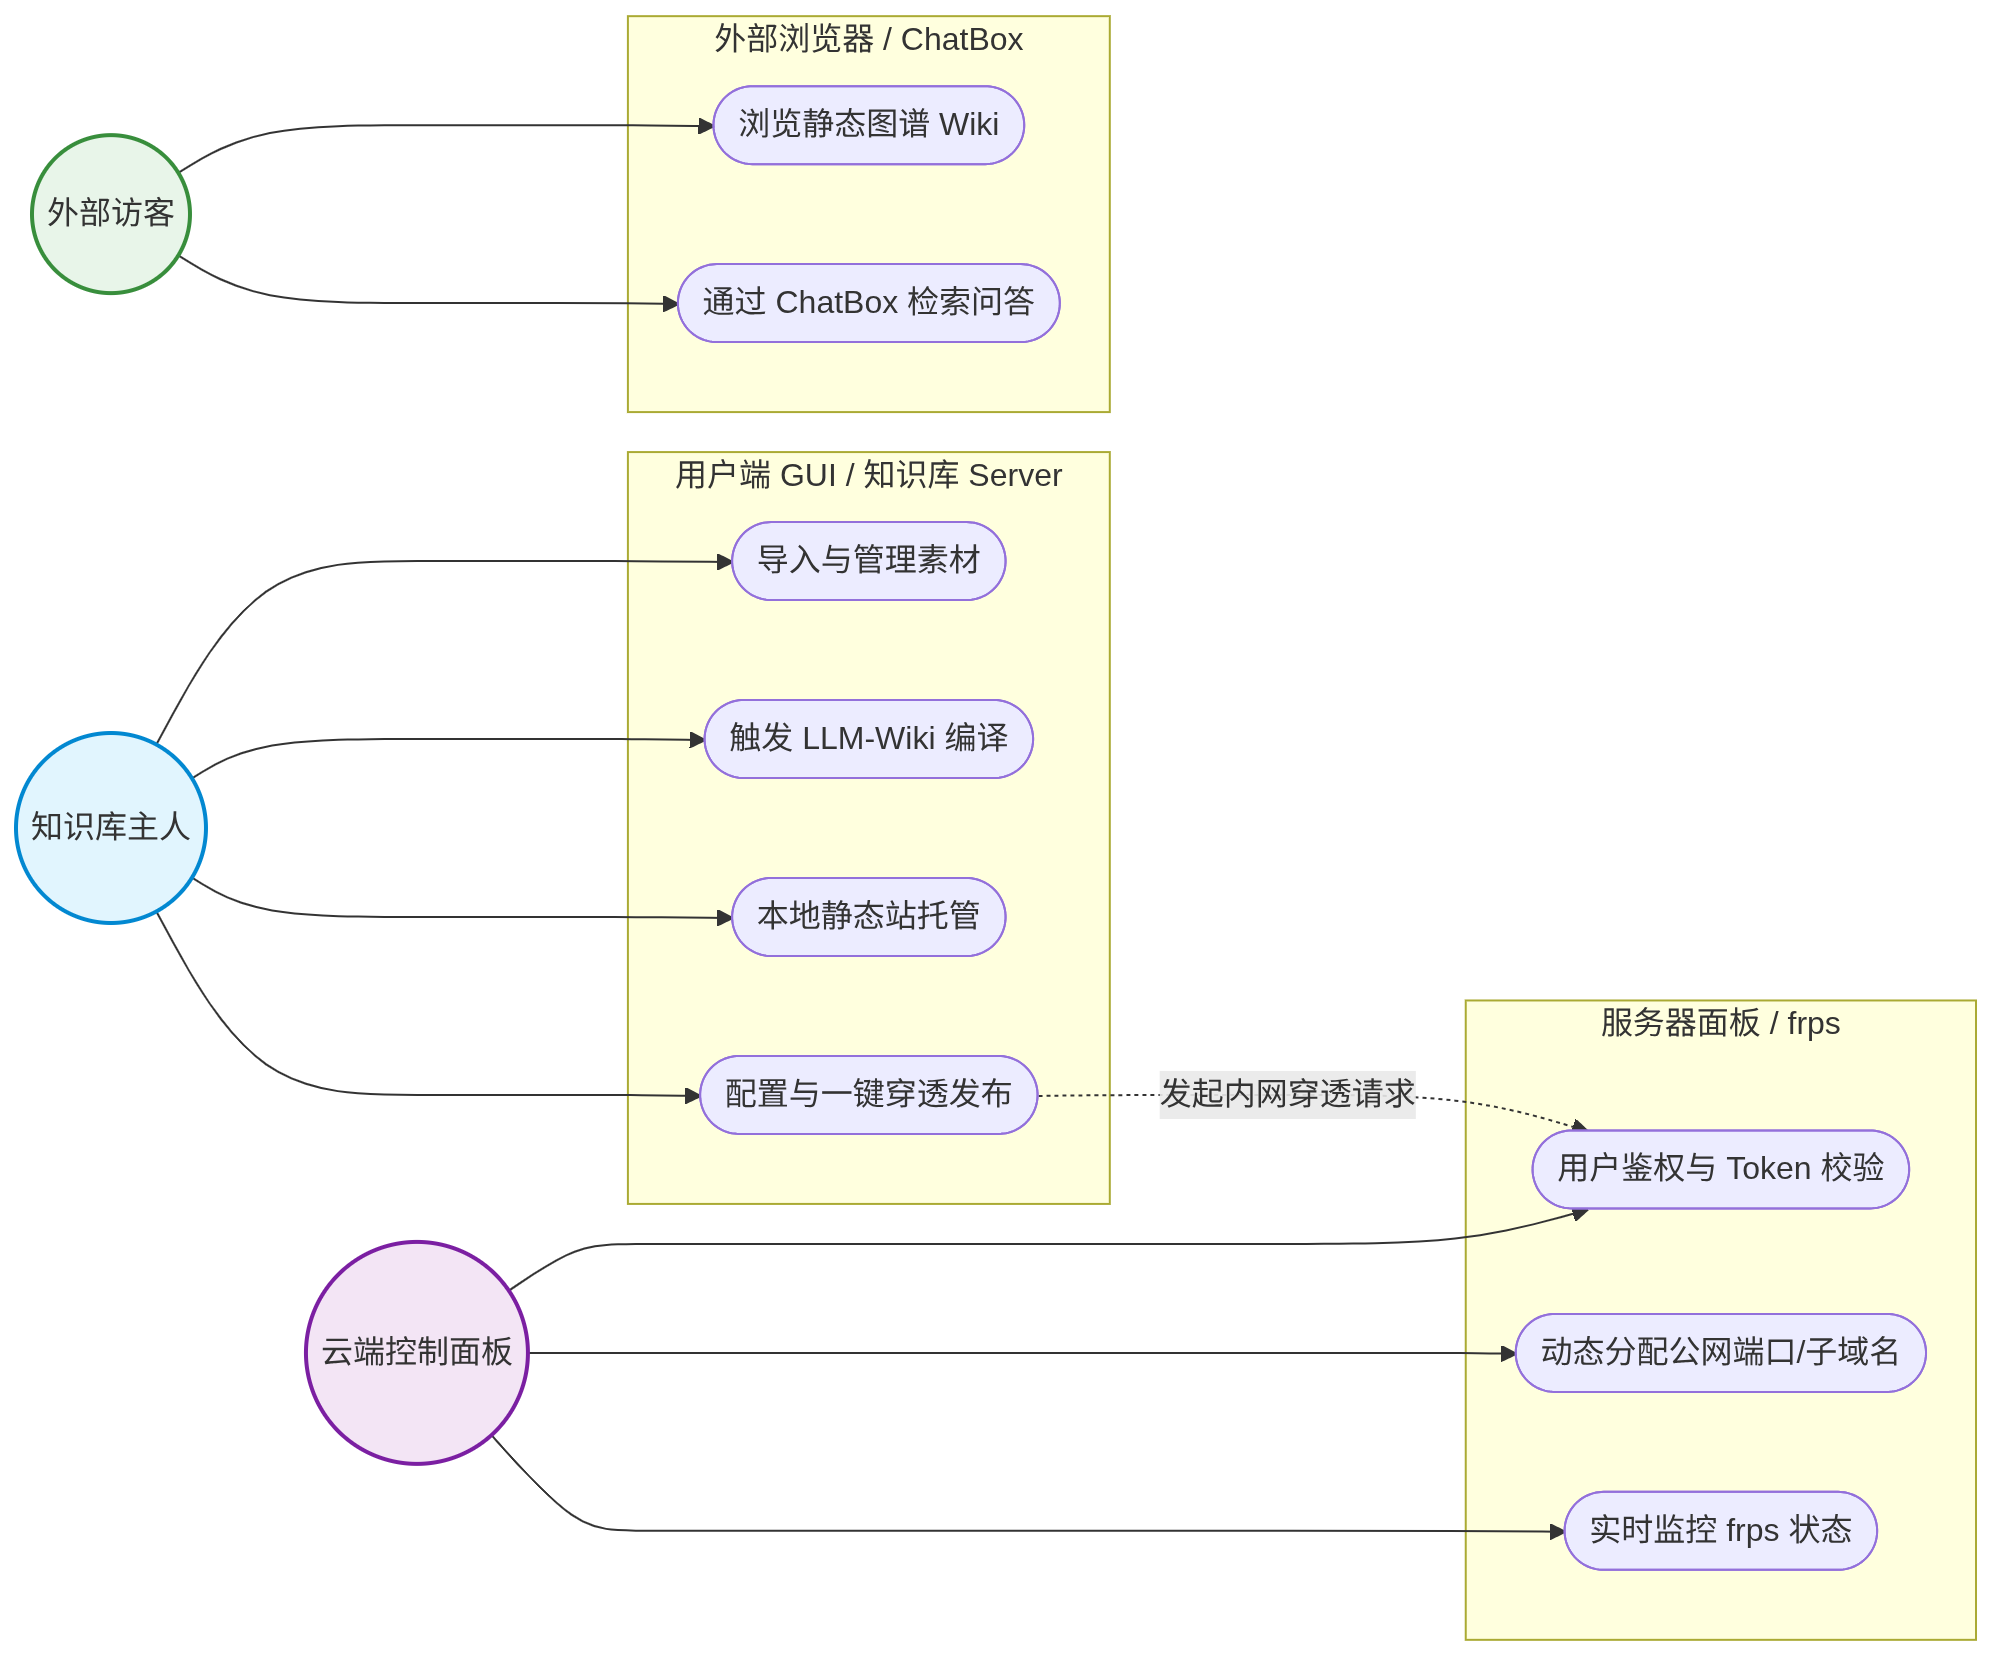
\includegraphics[height=0.78\textheight]{image/usecase_diagram.png}
    \end{figure}
\end{frame}

\begin{frame}{时序图：端到端发布与访问流程}
    \begin{figure}
        \centering
        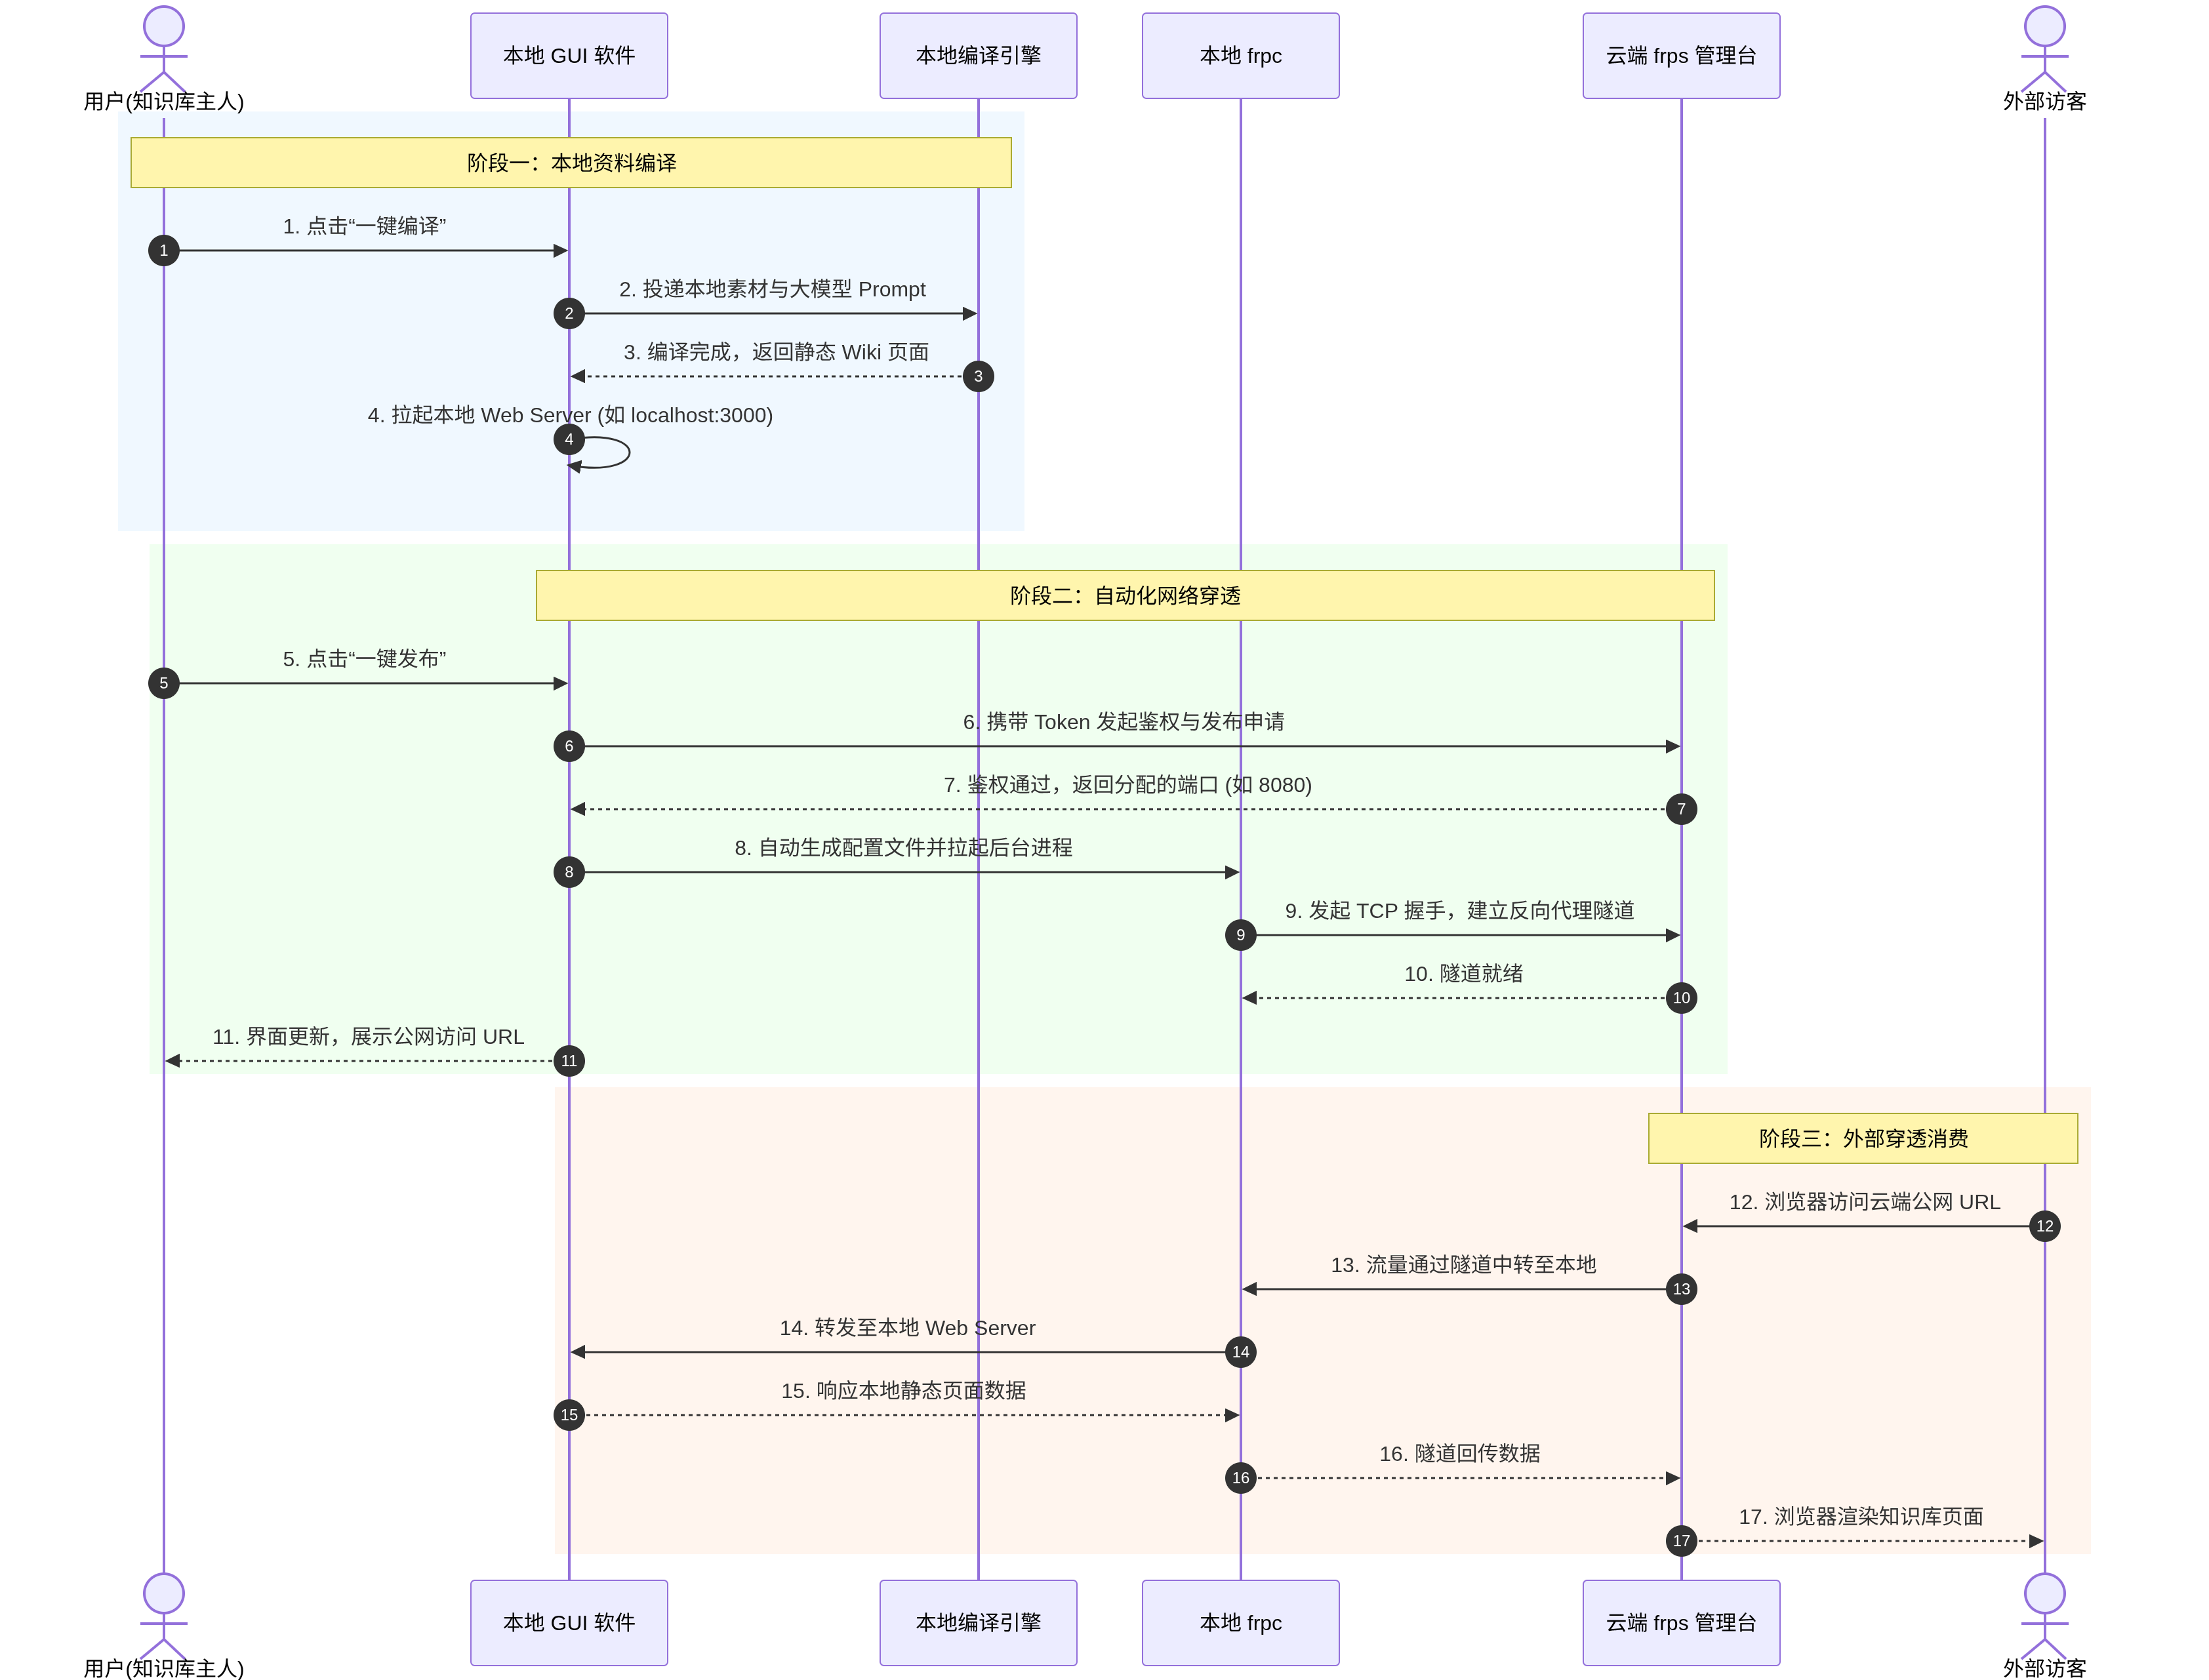
\includegraphics[width=0.92\linewidth]{image/sequence_diagram.png}
    \end{figure}
\end{frame}

\begin{frame}{非功能需求}
    \begin{itemize}
        \item \keypoint{易用性}：用户端尽量双击即用，不要求安装 Python、Docker 或手动配置命令行。
        \item \keypoint{隐私安全}：云端不存储用户笔记、文档、Wiki 页面或向量数据。
        \item \keypoint{低成本}：静态 Wiki 浏览不消耗 Token，只有编译、检查或问答时产生 AI 开销。
        \item \keypoint{可靠性}：编译失败、网络断开、端口占用时给出可理解的状态提示。
        \item \keypoint{可维护性}：知识库生成模块与 frp 管理模块解耦，便于后续扩展。
    \end{itemize}
\end{frame}

\begin{frame}{状态图：发布隧道生命周期与容错}
    \begin{figure}
        \centering
        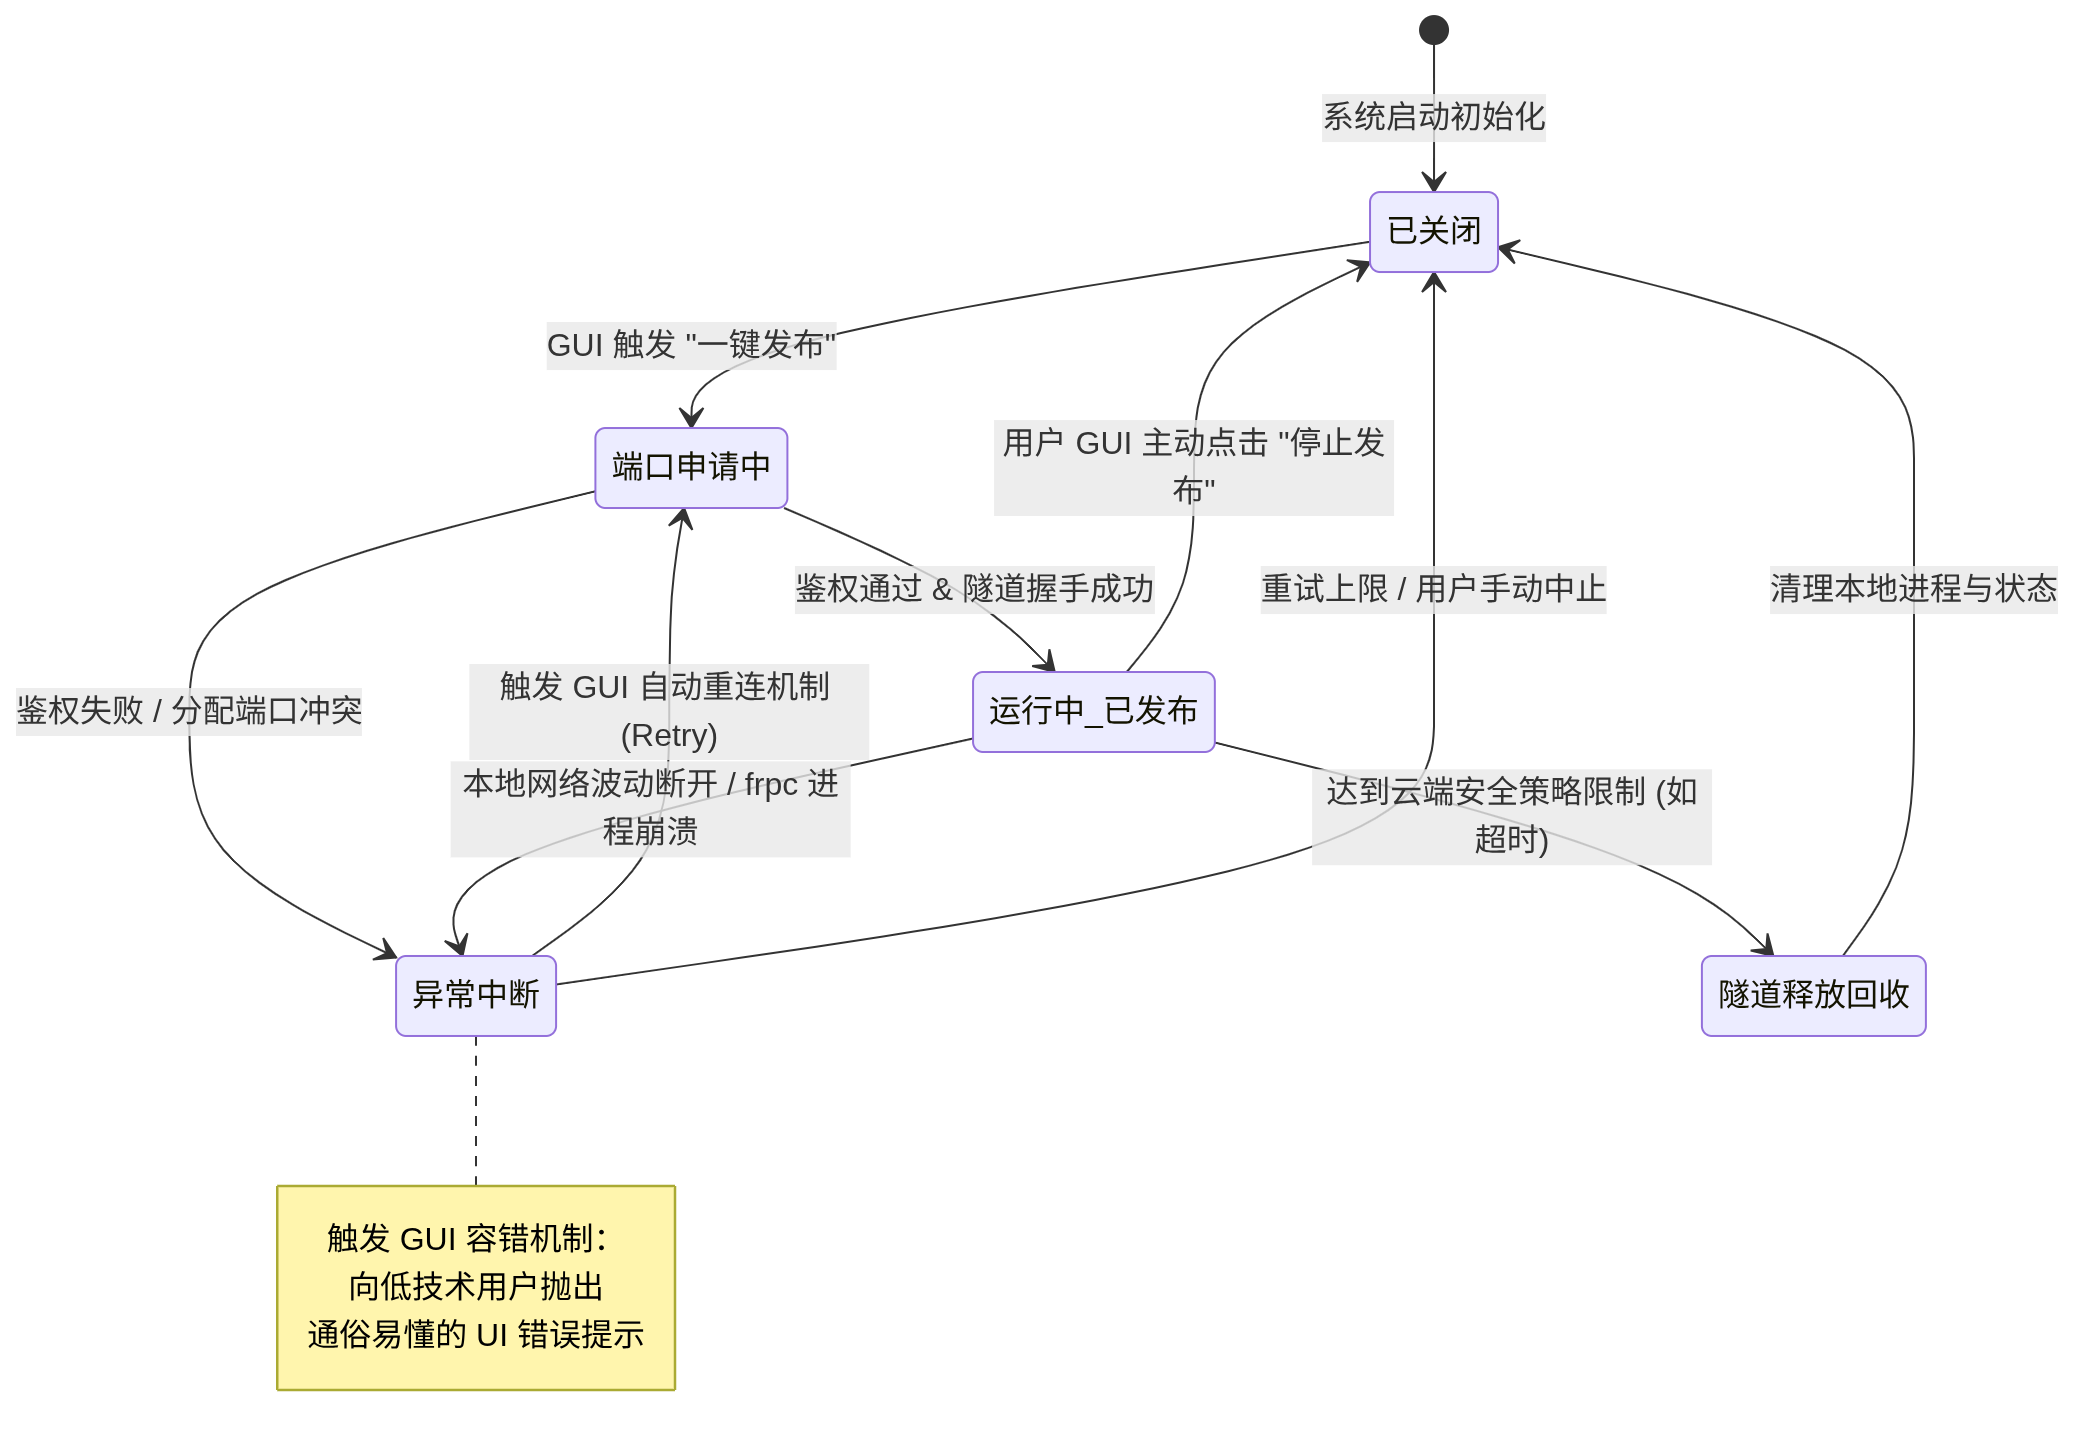
\includegraphics[height=0.78\textheight]{image/state_diagram.png}
    \end{figure}
\end{frame}

\section{项目开发计划}

\begin{frame}{3-4 周原型计划}
    \small
    \begin{tabularx}{\textwidth}{>{\raggedright\arraybackslash}p{0.16\textwidth}p{0.39\textwidth}X}
        \toprule
        \textbf{阶段} & \textbf{核心目标} & \textbf{关键输出物} \\
        \midrule
        第 1 周 & 明确角色、三端边界和核心流程。 & 需求说明、架构图、流程图、原型草图。 \\
        第 2 周 & 打通素材读取、Wiki 生成和本地渲染。 & 编译脚本、本地 Web Server、基础 Wiki 页面。 \\
        第 3 周 & 接入 frp、用户鉴权和公网 URL。 & frps / frpc 联调、公网演示地址。 \\
        第 4 周 & 完善日志、错误提示和 Lint 检查。 & 端到端原型、测试记录、阶段汇报 PPT。 \\
        \bottomrule
    \end{tabularx}
\end{frame}

\begin{frame}{阶段优先级}
    \begin{enumerate}
        \item \keypoint{先打通主链路}：从本地素材到 Wiki 页面，再到公网 URL 访问。
        \item \keypoint{再完善可控性}：账号、Token、端口、连接状态和访问入口可管理。
        \item \keypoint{最后优化体验}：减少用户配置，完善日志、错误提示和演示效果。
    \end{enumerate}

    \vspace{0.35cm}
    \begin{alertblock}{阶段一目标}
        验证“LLM-Wiki 本地编译 + frp 无感穿透”的端到端可行性。
    \end{alertblock}

    \vspace{0.25cm}
    \centering
    \Large 谢谢！
\end{frame}

\end{document}
